%%%% Better Poster latex template example v1.0 (2019/04/04)
%%%% GNU General Public License v3.0
%%%% Rafael Bailo
%%%% https://github.com/rafaelbailo/betterposter-latex-template
%%%% 
%%%% Original design from Mike Morrison
%%%% https://twitter.com/mikemorrison

\documentclass[a0paper,fleqn]{betterposter}


%% Setting the width of columns
% Left column from original 0.25
\setlength{\leftbarwidth}{0.27\paperwidth}
% Right column from original 0.25
\setlength{\rightbarwidth}{0.27\paperwidth}
\renewcommand{\fontsizemain}{\fontsize{115}{160} \selectfont}

\DeclareFontFamily{U}{skulls}{}
\DeclareFontShape{U}{skulls}{m}{n}{ <-> skull }{}
\newcommand{\skull}{\text{\usefont{U}{skulls}{m}{n}\symbol{'101}}}

\begin{document}	
\betterposter{
%%%%%%%% MAIN COLUMN

\maincolumn{
%%%% Main space

Banks should focus on analyzing \textbf{customer transaction history} and \textbf{activity} to accurately predict churn rather than user demographics. \\




\vfill


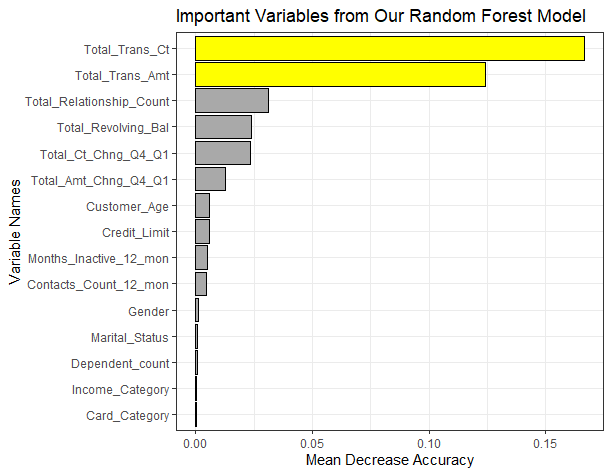
\includegraphics[width=\textwidth]{img/Rplot_2.5.png}\\ 



}{
%%%% Bottom space


}

}{
%%%%%%%% LEFT COLUMN

\title{Predicting Credit Card \\Customer Churn}
\author{Joseph Gallegos, Ajay Kallepalli, \\Lyndon Liang, Charles Liu, Anshuman Mahalley}



\section{Introduction}
As a competitive business, a bank would like to retain their existing customers and grow their customer base. To reduce the loss of customers (or churning), we seek to investigate variables that potentially influence customer behaviors and determine how the bank can minimize losses and optimize performance.


\section{Exploratory Data Analysis}
We started by modifying the character variables into factors to help with modeling. We also  decided to modify the economic class variable to simplify the process of determining people's Social Economic Status. We decided that lower income status would be "Less than \$40K", middle income would be "\$40K - \$60K" & "\$60K - \$80K", and high income would be "\$80K - \$120K" & "\$120K +". We then plotted this variable to see if there is significant difference between the economic classes from the attrited customers and existing customers. (seen below)

\section{Plot}
Plot for Economic class with attrited vs existing customers\\

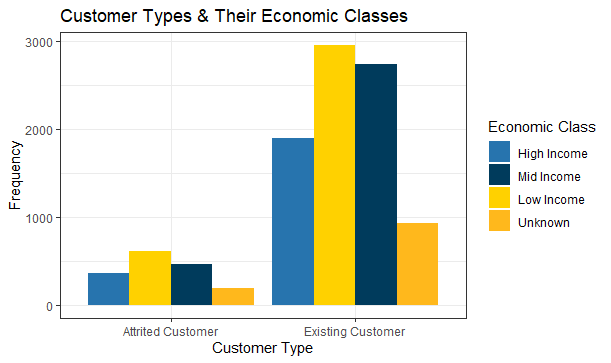
\includegraphics[width=\textwidth]{img/Rplot.png}\\ 


}{
%%%%%% RIGHT COLUMN
\section{Model Proposal}
We considered various classification methods like logistic regression, K Nearest Neighbors and random forest to predict which customers would churn. Our final model was a random forest model with the following variables listed in decreasing order of their MeanDecreaseAccuracy: Total\_Trans\_Ct, Total\_Trans\_Amt, Total\_Revolving\_Bal, Total\_Relationship\_Count, Avg\_Utilization\_Ratio etc. Hyperparameter tuning was done using grid search and our best performing model had parameters mtry = 15, ntree = 500 with an accuracy of 96.45%. 


\section{Conclusion}
We see from the model that there are certain variables that correspond to a customer being more likely to cancel their subscription. To maximize profit it would be best for a company to use this model to identify those customers that are most likely to churn and proactively try and improve their experience through better support or various other direct incentives. From our analysis we see that this prediction is best done by using customers credit card usage statistics instead of their demographics data. Ultimately there are numerous valuable and actionable insights that a company can glean from our presentation.\\

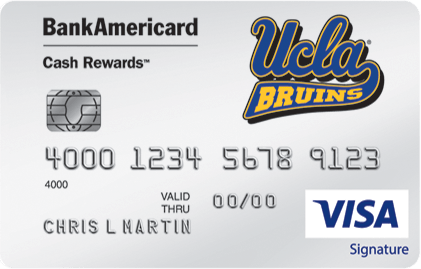
\includegraphics[width=0.47\textwidth]{img/UCLA-Credit-Card.png} \hspace{1.3cm}
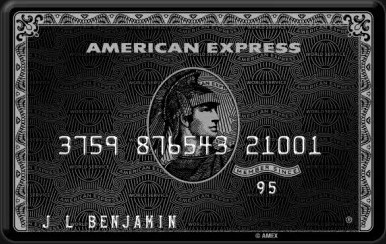
\includegraphics[width=0.47\textwidth]{img/black-card.jpg}
\begin{center}
    \caption{Customer's credit cards before and after the model!}
\end{center}



\section{References}
Data:\:https://www.kaggle.com/sakshigoyal7/credit-card-customers\\
Website:\:https://jfin-swufe.springeropen.com/articles/\\10.1186/s40854-016-0029-6



\vfill
\begin{center}
    
\includegraphics[width=0.5\textwidth]{img/DeptLogo.png}\\
\end{center}}

\end{document}
